\section {Capacitor Modeling}
\subsection{Statistics Review}
Capacitors can be represented by numerous equivalent-circuit models, which have various degrees of accuracy in representing the reponse of a physical system. Equivalent circuit models for capacitors usually have either individual or groups of terms that are  of interest for different applications. For instance, designers of switch-mode power supplies need to know the ESR of a capacitor in order to be able to use it for output filtering. When an unknown capacitor is characterized, its response to an electrical stimulous will be recorded and then analyzed. The resulting data is fit to a model using regression analysis. Using various statistical analysis tools, one can determine a model's effectiveness at describing a capacitor to either predict its behavior in a circuit or to compare it against other capacitors. This section will provide a brief introduction into the regression analysis techniques that are proposed in this paper to fit capacitor data to a model.

\begin{figure}
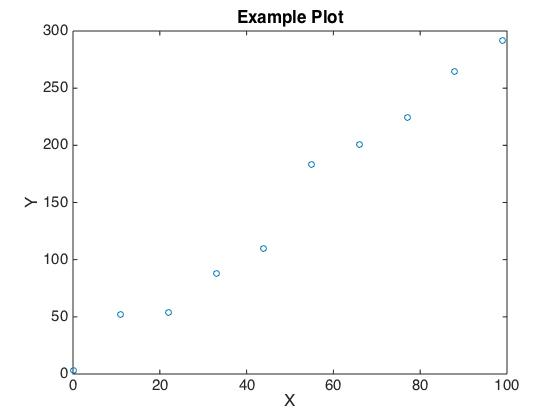
\includegraphics[keepaspectratio=true,width=6in]{./figures/modeling/exLinearData.jpg}
\centering
\caption{Example Data}
\label{fig:exLinearData}
\end{figure}


The basic task in regression analysis is to take a data set, such as shown in Figure: \ref{fig:exLinearData}, and find the equation of a line that reasonably fits the data. The first thing that we need to do is to choose the form of the line that we want to fit to the data. A good choice for the example at hand would be the line shown in Equation: \eqref{equ:ExLinEqu}. A commonly used regression analysis technique is called the Least Squares Estimate (LSE). It attempts to find a model which minimizes the squared error between an empirical set of data and itself (Equations: \eqref{equ:LSE_E2} \& \eqref{equ:LSE_E2b}).

\begin{equation}
\label{equ:ExLinEqu}
y = b_0 + b_1 x
\end{equation}

\begin{equation}
\label{equ:LSE_E2}
E^2 = \sum_{i=1}^{n} (y_i - y)^2
\end{equation}

\begin{equation}
\label{equ:LSE_E2b}
E^2 = \sum_{i=1}^{n} (y_i - (b_0 + b_1 x_i)^2
\end{equation}

In order to minimize the squared error over the data set, we need to take the partial derivate of Equation: \eqref{equ:LSE_E2b} with respect to each of the unknown parameters seperately. While $b_0$ and $b_1$ will be constants in the final equation, they are treated as variables here until they are known. Conversely, all $x_i$ values are treated as constants. This results in Equations: \eqref{equ:LSE_PD1} \& \eqref{equ:LSE_PD2}.

\begin{equation}
\label{equ:LSE_PD1}
\frac{\partial E^2}{\partial b_0} = 0 = \sum_{i=1}^{n} (-2y_i +2b_0 + 2b_1 x_i)
\end{equation}

\begin{equation}
\label{equ:LSE_PD2}
\frac{\partial E^2}{\partial b_1} = 0 = \sum_{i=1}^{n} (-2y_i x_i +2b_0 x_i + 2b_1 x_i^2)
\end{equation}

Up to this point most LSE analyses follow the same basic path. But the rest of the steps depend upon the complexity of the model and solution techniques. The following steps use transformations and substitutions to solve for the unknown variables. In our case, we can use Equations: \eqref{equ:avg} \& \eqref{equ:avgb} to remove the summation terms from the equation.

\begin{equation}
\label{equ:avg} 
\bar{y} = (\sum_{i=1}^{n} y_i) / n
\end{equation}

\begin{equation}
\label{equ:avgb} 
\sum_{i=1}^{n} y_i  = \bar{y}n
\end{equation}

This results in Equations: \eqref{equ:LSE_sol} \& \eqref{equ:LSE_solb} with solutions shown in Equations: \eqref{equ:LSE_solc} \& \eqref{equ:LSE_sold}. The empirical data is then used to find the values of $b_0$ and $b_1$. At this point, the line can be used to estimate new points on the plot or to compare against other data sets.

\begin{equation}
\label{equ:LSE_sol}
0 = \bar{y} - (b_0 + 2b_1 \bar{x})
\end{equation}

\begin{equation}
\label{equ:LSE_solb}
0 = \bar{xy} - (b_0 \bar{x} + 2b_1 \bar{x^2})
\end{equation}

\begin{equation}
\label{equ:LSE_solc}
b_0 = \bar{y} - b_1 \bar{x}
\end{equation}

\begin{equation}
\label{equ:LSE_sold}
b_1 = \frac{\bar{xy} - \bar{x}\bar{y}}{\bar{x^2} - \bar{x}^2}
\end{equation}

Levy \cite{levy} shows an extension of the simple LSE example that is valid for a genaric polinomial transfer function. This method is important because it not only allows for a complex-valued transfer functions, but it also prevents the nececcity of needing to rederive the system of equations for each new model. 

\begin{equation}
\label{equ:levy_Gs}
G(s) = \frac{A_0 + A_1 s + A_2 s^2 + ... + A_n s^n}{B_0 + B_1 s + B_2 s^2 + ... + B_n s^n}
~\cite{levy}[Eq.~3]
\end{equation}

Using Equation: \eqref{equ:levy_Gs} as the genaric model for the equation at hand, Levy shows that you can use Equations: \eqref{equ:Levy_L}, \eqref{equ:Levy_S}, \eqref{equ:Levy_T}, \& \eqref{equ:Levy_U} to simplify the series of partial derivates into a single matrix mtiplication equation shown in \eqref{equ:Levy_Ans}.

\begin{equation}
\label{equ:Levy_L}
\lambda _h = \sum_{k=0}^{m} \omega _k ^h
~\cite{levy}[Eq.~15]
\end{equation}

\begin{equation}
\label{equ:Levy_S}
S_h = \sum_{k=0}^{m} \omega _k ^h R_k
~\cite{levy}[Eq.~16]
\end{equation}

\begin{equation}
\label{equ:Levy_T}
T_h = \sum_{k=0}^{m} \omega _k ^h I_k
~\cite{levy}[Eq.~17]
\end{equation}

\begin{equation}
\label{equ:Levy_U}
U_h = \sum_{k=0}^{m} \omega _k ^h (R_k ^2 + I_k ^2)
~\cite{levy}[Eq.~18]
\end{equation}

\begin{equation}
\label{equ:Levy_Ans}
MN = C
~\cite{levy}[Eq.~20]
\end{equation}

Once you choose the number of terms needed for your model, you use Equations: \eqref{equ:Levy_M}, \eqref{equ:Levy_N}, \& \eqref{equ:Levy_C} along with the empirical data to solve for the coefficients.

\setcounter{MaxMatrixCols}{12} % Allows each row of M to fit on one line
\begin{equation}
\label{equ:Levy_M}
M = 
\begin{bmatrix}
\lambda _0 & 0          & -\lambda _2 &  0           & \lambda _4  & \cdots &  T_1    & S_2    & -T_3   & -S_4   &  T_5    & \cdots \\
0          & \lambda _2 & 0           & -\lambda _4  & 0           & \cdots & -S_2    & T_3    &  S_4   & -T_5   & -S_6    & \cdots \\
\lambda _2 & 0          & -\lambda _4 &  0           & \lambda _6  & \cdots &  T_3    & S_4    & -T_5   & -S_6   &  T_7    & \cdots \\
0          & \lambda _4 & 0           & -\lambda _6  & 0           & \cdots & -S_4    & T_5    &  S_6   & -T_7   & -S_8    & \cdots \\

\vdots     & \vdots     &  \vdots     & \vdots       & \vdots      &        &  \vdots & \vdots & \vdots & \vdots &  \vdots &        \\ 
T_1        & -S_2       & -T_3        &  S_4         & T_5         & \cdots &  U_2    & 0      & -U_4   &  0     &  U_6    & \cdots \\
S_2        &  T_3       & -S_4        & -T_5         & S_6         & \cdots &  0      & U_4    &  0     & -U_6   &  0      & \cdots \\
T_3        & -S_4       & -T_5        &  S_6         & T_7         & \cdots &  U_4    & 0      & -U_6   &  0     &  U_8    & \cdots \\
\vdots     & \vdots     &  \vdots     & \vdots       & \vdots      & \vdots &  \vdots & \vdots & \vdots & \vdots &  \vdots &        \\ 
\end{bmatrix}
~\cite{levy}[Eq.~21a]
\end{equation}

\begin{multicols}{2}
\begin{equation}
\label{equ:Levy_N}
N = 
\begin{bmatrix}
A_0 \\
A_1 \\
A_2 \\
A_3 \\
\vdots \\
B_1 \\
B_2 \\
B_3 \\
\vdots
\end{bmatrix}
~\cite{levy}[Eq.~21b]
\end{equation}

\begin{equation}
\label{equ:Levy_C}
C = 
\begin{bmatrix}
S_0 \\
T_1 \\
S_2 \\
T_3 \\
\vdots \\
0   \\
U_2 \\
0   \\
\vdots
\end{bmatrix}
~\cite{levy}[Eq.~21c]
\end{equation}
\end{multicols}

\subsection{Modeling}
This section will show how to use the method put forth in the previous section to determine the model parameters for several important capacitor models.

\subsubsection{RLC}
The RLC model, shown in Figue: \ref{fig:rlcModel}, is one of the simplest models used to describe a capacitor. It shows the basic low and high frequency characteristics, along with the capacitor's resonant point.

\begin{figure}[ht!]
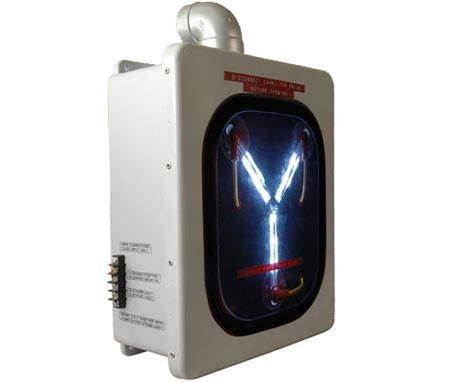
\includegraphics[keepaspectratio=true,width=2in]{./figures/regression/rlcModel.jpg}
\centering
\caption{RLC Model}
\label{fig:rlcModel}
\end{figure}


\begin{equation}
\label{equ:rlc_Zs}
Z(s) = R + sL + \frac{1}{sC}
\end{equation}

\begin{equation}
\label{equ:rlc_Zs2}
Z(s) = \frac{1 + s(RC) + s^2 (LC)}{sC}
\end{equation}

\begin{equation}
\label{equ:rlc_Zs3}
Z_2(s) = Z(s) * sC =  \frac{1 + s(RC) + s^2 (LC)}{1}
\end{equation}

\begin{equation}
\label{equ:rlc_Zs4}
Z_2(s) = \frac{A_0 + A_1 s + A_2 s^2}{B_0 + B_1 s + B_2 s^2}
\end{equation}

